\documentclass[crop,tikz]{standalone}

\tikzset{>=latex}
\usetikzlibrary{calc,decorations.markings,shapes}
\colorlet{gray}{gray!20}
\colorlet{green}{black!40!green}

\begin{document}
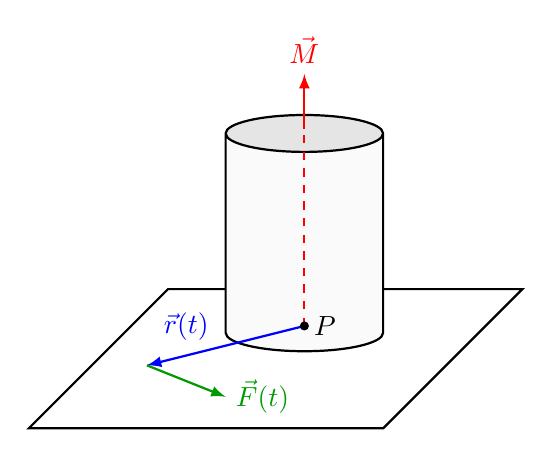
\begin{tikzpicture}
  \coordinate (C) at (0,-1);
  \coordinate (R) at ($(C)+(-2cm,-0.5cm)$);
  % plate
  \draw[thick] (-3.5cm,-2.3cm) -- ++(4.5cm,0) -- ++(45:2.5) -- ++(-4.5cm,0) -- cycle;
  % cylinder
  \node (A) at (0,0) [thick, cylinder, aspect=2, shape border rotate=90, draw, minimum height=3cm, minimum width=2cm, cylinder body fill=gray!20, cylinder uses custom fill, cylinder end fill=gray] {};
  % turning momentum
  \draw[dashed,red,thick] (C) -- ++(0,3-1/2) coordinate (M);
  \draw[->,red,thick] (M) -- +(0,0.7cm) node[above] {$\vec{M}$};
  \draw[->,blue,thick] (C) -- node[above,xshift=-0.5cm,yshift=-0.2em] {$\vec{r}(t)$} (R);
  \draw[->,green,thick] (R) -- +(1cm,-0.4cm) node[right] {$\vec{F}(t)$};
  \draw[fill] (C) circle (0.05cm) node[right] {$P$};
\end{tikzpicture}
\end{document}
